\documentclass[a0,landscape,pdftex]{a0poster}

\usepackage{amsthm,amsmath,amssymb,amsfonts,graphicx,algorithm,algorithmic}
\usepackage[scaled=1.1]{helvet}
\usepackage{postercols2}
\usepackage{flowfram}
\usepackage{color}
\usepackage{lipsum}
\usepackage{rotating}
\usepackage{subcaption}
\usepackage{booktabs}
\usepackage{multirow}
\usepackage{multicol}
\usepackage{paper_commands}


\setlength{\flowframesep}{.2in}
\setlength\parindent{0pt}
\setlength{\vcolumnsep}{.5in}
\setlength{\columnsep}{\vcolumnsep}

\Ncolumntop{static}{2}{3in}
\setstaticframe{1}{label={title}}

\newlength\offset
\setlength{\offset}{18.5in}
\addtolength{\offset}{\vcolumnsep}
\computeflowframearea{2}
\addtolength{\ffareaheight}{-\offset}
%\setflowframe{2}{height=\ffareaheight}
\addtolength{\ffareaheight}{\vcolumnsep}
%\newstaticframe{\ffareawidth}{18.5in}{\ffareax}{\ffareaheight}[figures]
\setstaticframe{20}{clear}

%this puts borders on the frames
%\setallflowframes{border=plain}
%\setallstaticframes{border=plain}

\title{Disentangling and Integrating Relational and Sensory Information in Transformer Architectures}
%\author{}
\date{}


\begin{document}

\begin{staticcontents*}{title}
\maketitle
\end{staticcontents*}
\thispagestyle{empty}

\Large

\section*{Relational games}

\begin{minipage}{55cm}

We computed learning curves on relational games, comparing \textit{DAT} against multiple Transformer baselines of varying sizes and architectural hyperparameters (e.g., \# of heads). We also 
computed learning curves on relational games, comparing \textit{DAT} against PrediNet, CoRelNet, Abstractor, and Transformer baselines.


\begin{center}
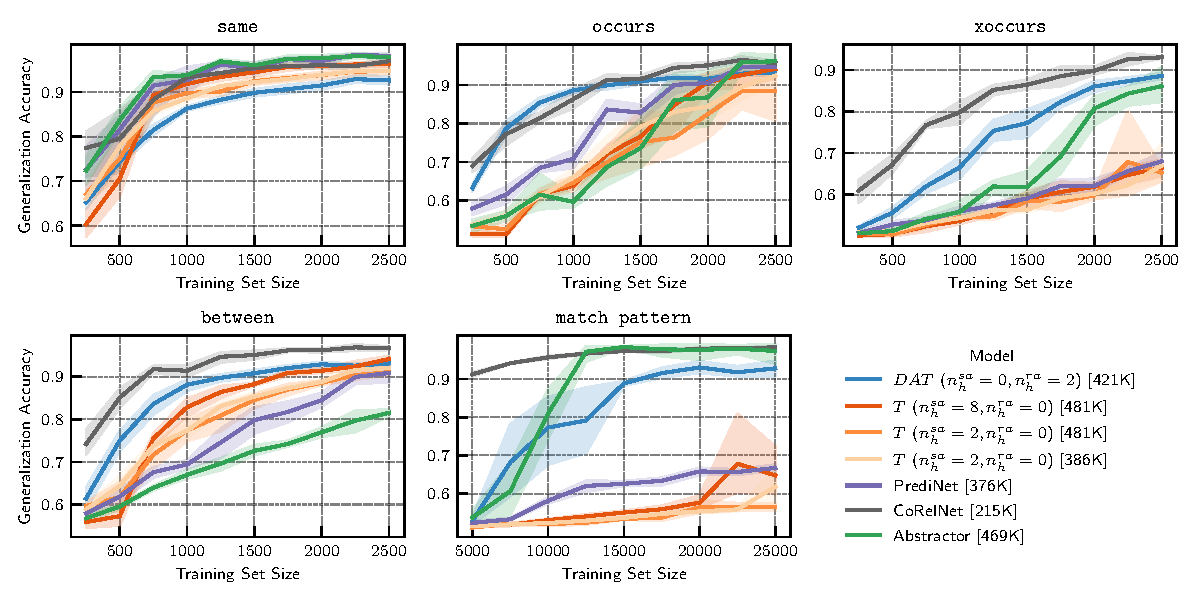
\includegraphics[width=0.95\textwidth]{../figs/experiments/relgames/relgames_learning_curves_baseline_comparisons.pdf}
\end{center}


\section*{Mathematics processing}


Validation accuracy over the course of training for seq2seq mathematical problem-solving:

% maybe pick one of the two 
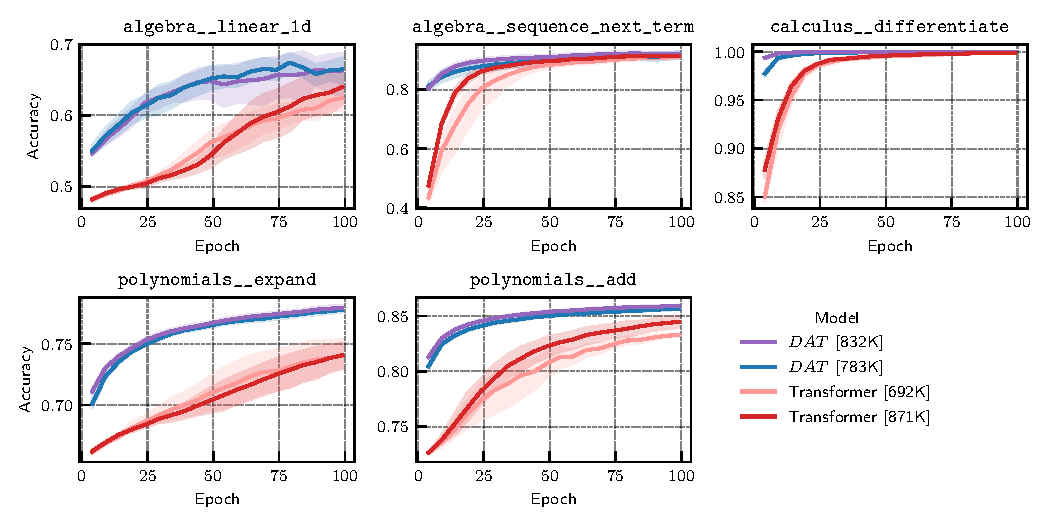
\includegraphics[width=0.95\textwidth]{../figs/experiments/math/math_training_curves_interpolation.pdf}
\end{minipage}

\begin{minipage}{55cm}

We also ran sequence-to-sequence symbolic mathematical processing, comparing to a Transformer at multiple scales, with \textit{DAT} models of model dimension $128$ and Transformer models of model dimension $144$, with three models each with 2, 3, or 4 layers. Superiority of \textit{DAT} persists across all depths and model sizes. Figures included in revised paper.


\section*{Language modeling at larger scale}

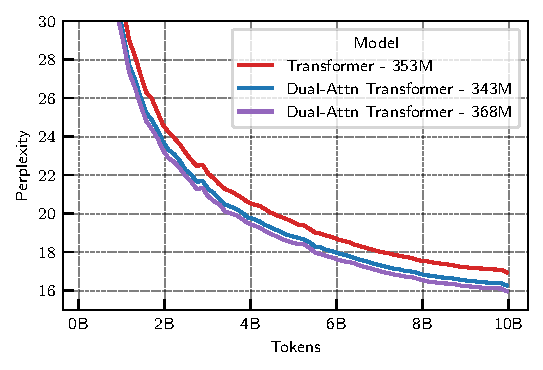
\includegraphics[width=.50\textwidth]{../figs/experiments/fineweb/350M_scale_lm.pdf}
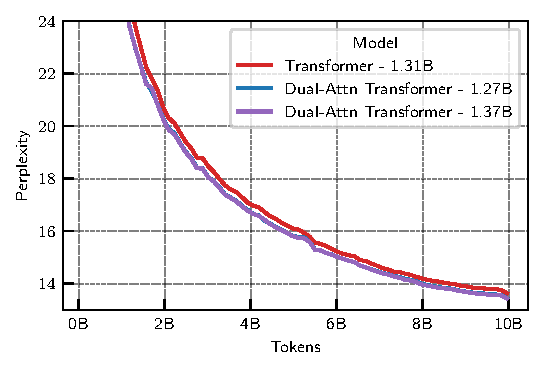
\includegraphics[width=.50\textwidth]{../figs/experiments/fineweb/1_3B_scale_lm.pdf}

Plots show perplexity curves on language modeling with the Fineweb dataset. The $x$-axis indicates the number of tokens and the $y$-axis is the validation perplexity. \textit{DAT} learns faster and achieves smaller perplexity at multiple model size scales.

\vskip2cm
\begin{center}
% \begin{tabular}{@{}l|ccccccc|c@{}}
\begin{tabular}{@{}lcc|cccccc|c@{}}
    \toprule
    Model        & Param count   & \# Tokens &$\dmodel$&$\nlayers$& $\nhsa$  & $\nhra$ & $d_r$ & $n_{kv}^{h}$ & Perplexity $\downarrow$ \\ \midrule\hline
    Transformer  & 353M   & 10B       & 1024    & 24       & 16       & -        & -     & -           & 16.94     \\
    \textit{DAT} & 343M   & 10B       & 1024    & 24       & 8        & 8        & 8    & 4           & 16.26     \\
    \textit{DAT} & 343M   & 10B       & 1024    & 24       & 8        & 8        & 32    & 4           & 16.14     \\
    \textit{DAT} & 343M   & 10B       & 1024    & 24       & 8        & 8        & 64    & 4           & 16.09     \\
    % \textit{DAT} & 368M   & 10B       & 1024    & 24       & 8        & 8        & 8   & 8           & 15.97     \\\midrule
    Transformer  & 1.31B  & 10B       & 2048    & 24       & 32       & -        & -     & -           & 13.63     \\
    \textit{DAT} & 1.27B  & 10B       & 2048    & 24       & 16       & 16       & 64    & 8           & 13.44     \\
    \textit{DAT} & 1.37B  & 10B       & 2048    & 24       & 16       & 16       & 64    & -          & 13.43     \\ \bottomrule
    % Model / Param count   &$\dmodel$&$\nlayers$& $\nhsa$  & $\nhra$ & $n_r$ & $n_{kv}^{h}$ & Perplexity $\downarrow$ \\ \midrule\hline
    % Transformer - 353M   & 1024    & 24       & 16       & -        & -     & -           & 16.944     \\
    % \textit{DAT} - 343M  & 1024    & 24       & 8        & 8        & 32    & 4           & 16.258     \\
    % \textit{DAT} - 368M  & 1024    & 24       & 8        & 8        & 32    & 8           & 15.969     \\\midrule
    % Transformer - 1.31B  & 2048    & 24       & 32       & -        & -     & -           & 13.630     \\
    % \textit{DAT} - 1.27B & 2048    & 24       & 16       & 16       & 64    & 8           & 13.440     \\
    % \textit{DAT} - 1.37B & 2048    & 24       & 16       & 16       & 64    & 16          & 13.426     \\ \bottomrule
\end{tabular}%
    % }
    % & $n_s$ 
    % & -     
    % & 1024  
    % & 1024  
    % & -     
    % & 512   
    % & 2048  
\end{center}

\end{minipage}


\end{document}
